\documentclass{standalone}
\usepackage{tikz}
\usetikzlibrary{positioning}
\begin{document}
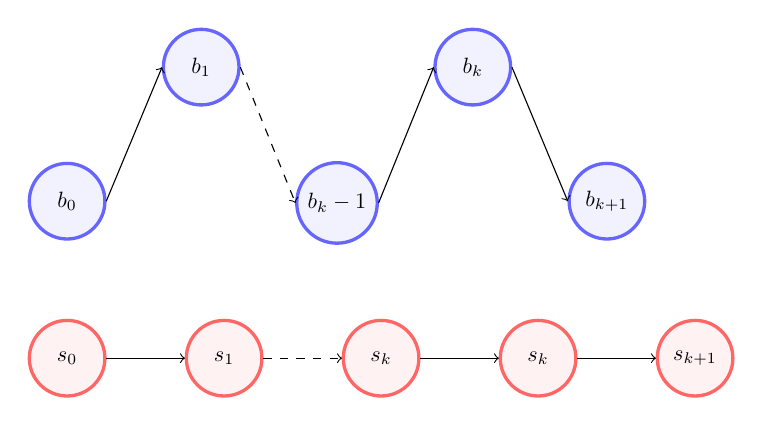
\begin{tikzpicture}[
beliefnode/.style={circle, draw=blue!60, fill=blue!5, very thick, minimum size=12mm},
rabinnode/.style={circle, draw=red!60, fill=red!5, very thick, minimum size=12mm}, every node/.style={scale=0.8}
]
% Belief path
%Nodes
\node[beliefnode]        (b0)                     {$b_0$};
\node[beliefnode]        (b1)       [above right=of b0] {$b_1$};
\node[beliefnode]        (b2)       [below right=of b1] {$b_k-1$};
\node[beliefnode]        (b3)       [above right=of b2] {$b_k$};
\node[beliefnode]        (b4)       [below right=of b3] {$b_{k+1}$};
%Lines
\draw[->] (b0.east) -- (b1.west);
\draw[dashed,->] (b1.east) -- (b2.west);
\draw[->] (b2.east) -- (b3.west);
\draw[->] (b3.east) -- (b4.west);
% Rabin Path
%Nodes
\node[rabinnode]        (s0)        [below=of b0]   {$s_0$};
\node[rabinnode]        (s1)        [right=of s0]   {$s_1$};
\node[rabinnode]        (s2)        [right=of s1]   {$s_k$};
\node[rabinnode]        (s3)        [right=of s2]   {$s_k$};
\node[rabinnode]        (s4)        [right=of s3]   {$s_{k+1}$};
%Lines
\draw[->] (s0.east) -- (s1.west);
\draw[dashed,->] (s1.east) -- (s2.west);
\draw[->] (s2.east) -- (s3.west);
\draw[->] (s3.east) -- (s4.west);


\end{tikzpicture}
\end{document}

